
%(BEGIN_QUESTION)
% Copyright 2007, Tony R. Kuphaldt, released under the Creative Commons Attribution License (v 1.0)
% This means you may do almost anything with this work of mine, so long as you give me proper credit

Since the outlet temperature of a heat exchanger can only change if there is an imbalance of inlet and outlet heat rates (assuming constant liquid inlet temperature and constant liquid composition), would this system be practical to achieve steady liquid outlet temperature control?  Explain why or why not.

$$\includegraphics[width=15.5cm]{i01770x01.eps}$$

Note: the philosophy behind this control system is a principle known as {\it energy balance}, and it is a very valid principle.  Explain what the principle of ``energy balance'' is, and how it is implied in the design of this control system.

\vskip 20pt \vbox{\hrule \hbox{\strut \vrule{} {\bf Suggestions for Socratic discussion} \vrule} \hrule}

\begin{itemize}
\item{} A powerful problem-solving technique is performing a {\it thought experiment} where you mentally simulate the response of a system to some imagined set of conditions.  Describe a useful ``thought experiment'' for this system, and how the results of that thought experiment are helpful to answering the question.
\item{} Explain why the control system as shown is impractical for real-life use, despite the fact that it does represent a very effective and important control strategy frequently used in industry.
\item{} Determine whether the controller needs to be {\it direct} acting or {\it reverse} acting.
\item{} A problem-solving technique useful for analyzing control systems is to mark the PV and SP inputs of all controllers with ``+'' and ``$-$'' symbols, rather than merely label each controller as ``direct'' or ``reverse'' action.  Apply this technique to the control strategy shown here, identifying which controller input(s) should be labeled ``+'' and which controller input(s) should be labeled ``$-$''.
\item{} Modify this control strategy to incorporate ``feedback trim'' in addition to the feedforward action it currently possesses.
\item{} Are there any loads unaccounted for in this feedforward control strategy?  If so, see if you can modify this control strategy to account for them as well.
\end{itemize}

\underbar{file i01770}
%(END_QUESTION)





%(BEGIN_ANSWER)

In theory, this {\it feedforward} system would work to hold the liquid outlet temperature absolutely constant, because it will try to maintain heat flow out equal to heat flow in (energy out {\it balances} energy in).  However, there are some practical reasons why it would not work (even if the liquid inlet temperature and composition were held constant).

%(END_ANSWER)





%(BEGIN_NOTES)

One un-monitored load is the steam supply.  If the pressure and/or temperature varied, the amount of heat carried by any given flow rate would vary.  This in turn would cause temperature control errors unpredicted (and therefore uncompensated) by the feedforward system.

But even if we held the steam temperature and pressure constant, the system would remain impractical.  Variations in ambient temperature would change the parasitic heat load on the system, thus causing errors in temperature control.  Miscalibrations in one or both flowmeters would lead to temperature control errors as well.

\vfil \eject

\noindent
{\bf Prep Quiz:}

{\it Energy balance} is a phrase meaning \underbar{what} in the context of process control?

\begin{itemize}
\item{} When the total energy output by a process is precisely equal to setpoint
\vskip 5pt 
\item{} When all the overshoots of setpoint balance out all the undershoots of setpoint
\vskip 5pt 
\item{} When the total energy flowrate in equals the total energy flowrate out
\vskip 5pt 
\item{} When the output signal of a loop controller is equal to the input (PV) signal
\vskip 5pt 
\item{} The precise measurement of energy using a balance-scale instrument
\vskip 5pt 
\item{} It is a synonym for {\it motion-balance} when referencing pneumatic instruments
\end{itemize}

%INDEX% Control, strategies: feedforward
%INDEX% Process: heat exchanger temperature/flow control (generic)

%(END_NOTES)


